%%%%%%%%%%%%%%%%%%%%%%%%%%%%%%%%%%%%%%%%%%%%%%%%%%%%%%%%%%%%%%%%%%%%%%%%
\chapter{Results}
\label{sec:results}
%%%%%%%%%%%%%%%%%%%%%%%%%%%%%%%%%%%%%%%%%%%%%%%%%%%%%%%%%%%%%%%%%%%%%%%%

This chapter presents the main results of the porting effort. In particular, Section \ref{sec:it-works} covers algorithm-level compatibility. Section \ref{sec:performance-comparison} compares performance of the reference and the ported implementations on a number of different configurations of the Lyra2 algorithm. Finally, Section \ref{sec:mobile-application} demonstrates the ease of integration of the ported project into an Android mobile application.

\section{Algorithm-level Compatibility}
\label{sec:it-works}

The primary goal of this work was to port Lyra2 to Java so that it would produce the same hash values as the reference implementation when given the same inputs. Such algorithm-level compatibility was achieved and will be demonstrated in Section \ref{sec:manual-testing} and Section \ref{sec:automated-testing}. The former deals with hand-picked test vectors while the latter demonstrates a reasonably large collection of randomly picked test vectors and a unit-testing framework which uses them to verify hash results.

\subsection{Configuration Choice}
By design Lyra2 has a large number of configurable parameters. This section will provide the reasoning behind the choice of particular values. The short summary can be found in \autoref{table:configuration-summary}.

There are three sponges that could be tested: Blake2b, BlaMka and half-round BlaMka. Only the first two are in the manual testing shortlist because half-round BlaMka is similar to BlaMka. The sponge block size can be either 8, 10 or 12, so the extreme values made it into the shortlist. The columns of the memory matrix can be any positive number. The \path{Lyra2/src/runBenchCPU.sh} benchmarking script as well as other sources suggest that the values of 256 and 512 should be chosen.

Finally, time and memory costs are fixed at an arbitrary value of 100. The output length is chosen to be 10 so that the resulting hash value would fit easily on the page.

\begin{table}
\begin{center}
\begin{tabular}{l r}
Parameter & Value \\ \hline
Sponge & Blake2b, BlaMka \\
Sponge blocks & 8, 12 \\
Sponge rounds & 12 \\
Columns in the memory matrix & 256, 512 \\
Time cost (number of iterations) & 100 \\
Memory cost (number of rows in the memory matrix) & 100 \\
Output length (bytes) & 10 \\
\end{tabular}
\end{center}
\caption{Summary of parameter values for manually tested configurations}
\label{table:configuration-summary}
\end{table}

\subsection{Manual Testing}
\label{sec:manual-testing}

\autoref{fig:manual-testing} shows a log of manual tests. New line delimits different Lyra2 configurations. The first line of each group represents a particular configuration group: \verb|--outlen| is the output length, \verb|--tcost| is the time cost, \verb|--mcost| is the memory cost. The second and the forth line in each group is the password and salt pair, and the third and fifth lines are the resulting hash values.

\begin{code}
\begin{minted}[fontsize=\footnotesize]{shell}
$ lyra2 --sponge blake2b --blocks 8 --columns 256 --outlen 10 --tcost 100 --mcost 100
> "password" "salt"
> 19 FD 3B 50 9A 03 0C DF 95 DA
> "The quick brown fox jumped over the lazy dog" "0123456789"
> 04 A0 BF 30 D1 E5 A5 05 53 E9

$ lyra2 --sponge blake2b --blocks 8 --columns 512 --outlen 10 --tcost 100 --mcost 100
> "password" "salt"
> 73 39 79 B6 C1 3C C1 F3 D7 17
> "The quick brown fox jumped over the lazy dog" "0123456789"
> A1 B0 18 F6 B6 79 5F E0 2A A4

$ lyra2 --sponge blake2b --blocks 12 --columns 256 --outlen 10 --tcost 100 --mcost 100
> "password" "salt"
> 9C 52 2A B9 18 30 F9 E7 09 55
> "The quick brown fox jumped over the lazy dog" "0123456789"
> 7D B2 9D C8 31 B4 E9 0E 10 22

$ lyra2 --sponge blake2b --blocks 12 --columns 512 --outlen 10 --tcost 100 --mcost 100
> "password" "salt"
> AC F2 B6 50 2D BC F0 62 DD 29
> "The quick brown fox jumped over the lazy dog" "0123456789"
> 4F 1B 03 6B C9 A2 09 C4 BC DA

$ lyra2 --sponge blamka --blocks 8 --columns 256 --outlen 10 --tcost 100 --mcost 100
> "password" "salt"
> 53 32 F3 D7 C4 9C 46 38 3C 1B
> "The quick brown fox jumped over the lazy dog" "0123456789"
> E7 6E 4B A0 81 B8 3C CF D6 64

$ lyra2 --sponge blamka --blocks 8 --columns 512 --outlen 10 --tcost 100 --mcost 100
> "password" "salt"
> D9 F9 F5 65 0D 05 88 D0 DF F6
> "The quick brown fox jumped over the lazy dog" "0123456789"
> 3A 3D 40 00 3E 33 44 45 B3 DD

$ lyra2 --sponge blamka --blocks 12 --columns 256 --outlen 10 --tcost 100 --mcost 100
> "password" "salt"
> C1 BC 48 80 99 1C E7 E6 52 18
> "The quick brown fox jumped over the lazy dog" "0123456789"
> 2E 4E 56 C7 5B 3D B7 F9 E0 30

$ lyra2 --sponge blamka --blocks 12 --columns 512 --outlen 10 --tcost 100 --mcost 100
> "password" "salt"
> 82 AF EB 03 5B E7 12 11 BE 63
> "The quick brown fox jumped over the lazy dog" "0123456789"
> F7 A8 56 D5 81 16 AA E5 C7 4D
\end{minted}
\caption{Manual testing protocol, each configuration starts with \texttt{\$}, each password and salt pair is followed by the resulting hash value. The hash value is printed in hexadecimal.}
\label{fig:manual-testing}
\end{code}

\subsection{Automated Testing}
\label{sec:automated-testing}

The automated testing is possible because of the additional code that was added to the reference implementation. As mentioned in Section \ref{sec:reference-implementation}, there is a \verb|harness| branch which could be found in the forked GitHub project \cite{github:2017:lyra-copy} and the corresponding pull request \cite{github:2017:lyra-pr}. This branch introduces the \verb|Lyra2/tests/harness.py| script written in Python 3 which allows to compile several configurations of Lyra2 and then use those to compute and store hash values.

Additionally, the \verb|Lyra2/tests/take.py| Python 3 script was used to choose a number of random hash values from those previously precomputed. These were then used in the Java project to unit-test the implementation. Some of the hash values were also included into the continuous integration service and their status can be verified by visiting \cite{travis:2017:lyra}. However, continuous integration runs only a subset of the vectors that were run locally due to the limited amount of memory available on the remote machines. In conclusion, both manual and automated testing indicate that the ported implementation does not contain immediately visible problems.

\section{Performance Comparison}
\label{sec:performance-comparison}

The single-threaded configuration of the reference C implementation was compared to its ported Java counterpart. For that, a separate GitHub repository was set up in \cite{github:2017:lyra2-compare}. This repository needs to control software written in both C and Java which is why an expressive, high-level scripting language was chosen to complete this task: Python 3.

\subsection{Project Structure}

The comparison project \cite{github:2017:lyra2-compare} is a combination of two Jupyter Notebooks \cite{jupyter:2017:jupyter} and an SQlite database. The two created notebooks follow the producer-consumer strategy. The \mintinline{shell}{src/compare.ipynb} is the producer notebook which is responsible for compiling both C and Java implementations as well as dispatching computation tasks. The results are then collected into the \mintinline{shell}{measurements.db} SQLite database (which also serves as a cache layer). The consumer is the \mintinline{shell}{src/plot.ipynb} notebook which reads the data from the SQLite database and plots the figures shown below.

Lyra2 provides two main adjustable parameters: time and memory cost. Changing both of the parameters at the same time cannot be easily shown on a single graph which is why the comparison contains three main parts. Section \ref{sec:fixed-time-cost} and Section \ref{sec:fixed-memory-cost} show how several Lyra2 configurations behave when time cost and memory cost is fixed, respectively. Section \ref{sec:no-fixed-costs} shows a grid of values for both time and memory costs. In all the sections, the two projects are compared using four configurations:

\begin{itemize}
    \item Blake2b sponge with 256 columns, figures \ref{figure:mcost_256}, \ref{figure:tcost_256} and \ref{figure:tcost_mcost_blake2b_256}
    \item Blake2b sponge with 2048 columns, figures \ref{figure:mcost_2048}, \ref{figure:tcost_2048} and \ref{figure:tcost_mcost_blake2b_2048}
    \item BlaMka sponge with 256 columns, figures \ref{figure:mcost_256}, \ref{figure:tcost_256} and \ref{figure:tcost_mcost_blamka_256}
    \item BlaMka sponge with 2048 columns, figures \ref{figure:mcost_2048}, \ref{figure:tcost_2048} and \ref{figure:tcost_mcost_blamka_2048}
  \end{itemize}

Configurations were run in parallel, creating one process per configuration. Running time was measured as the time between process creation and its termination. Memory consumption was recorded from the parent process and its peak value was stored. For more details, please consult the \texttt{src/compare.ipynb} and \texttt{src/plot.ipynb} notebooks from \cite{github:2017:lyra2-compare}.

Finally, in Section \ref{sec:no-fixed-costs} the grid of time and memory cost parameters is \(200 \times 200\) with a step of \(10\), which results in a total of \(8 \times 21 \times 21 = 3528\) measurements used to build all the graphics.

\subsection{Fixed Time Cost}
\label{sec:fixed-time-cost}

There are two figures that show how running time and consumed memory depend on memory cost when time cost is fixed. Figure \ref{figure:mcost_256} shows a 256-column and figure \ref{figure:mcost_2048} shows a 2048-column configuration of Lyra2. Both these figures show that the reference implementation works faster and consumes less memory than its Java counterpart. A nice property is that both the running time and memory consumption are changing roughly linearly as the memory cost parameter is changed. This is consistent with the fact that the memory cost parameter corresponds to the number of rows of the in-memory matrix. There are some outliers with respect to both running time and memory consumption which can be attributed to different system loads.

\begin{figure}[H]
    \centering
    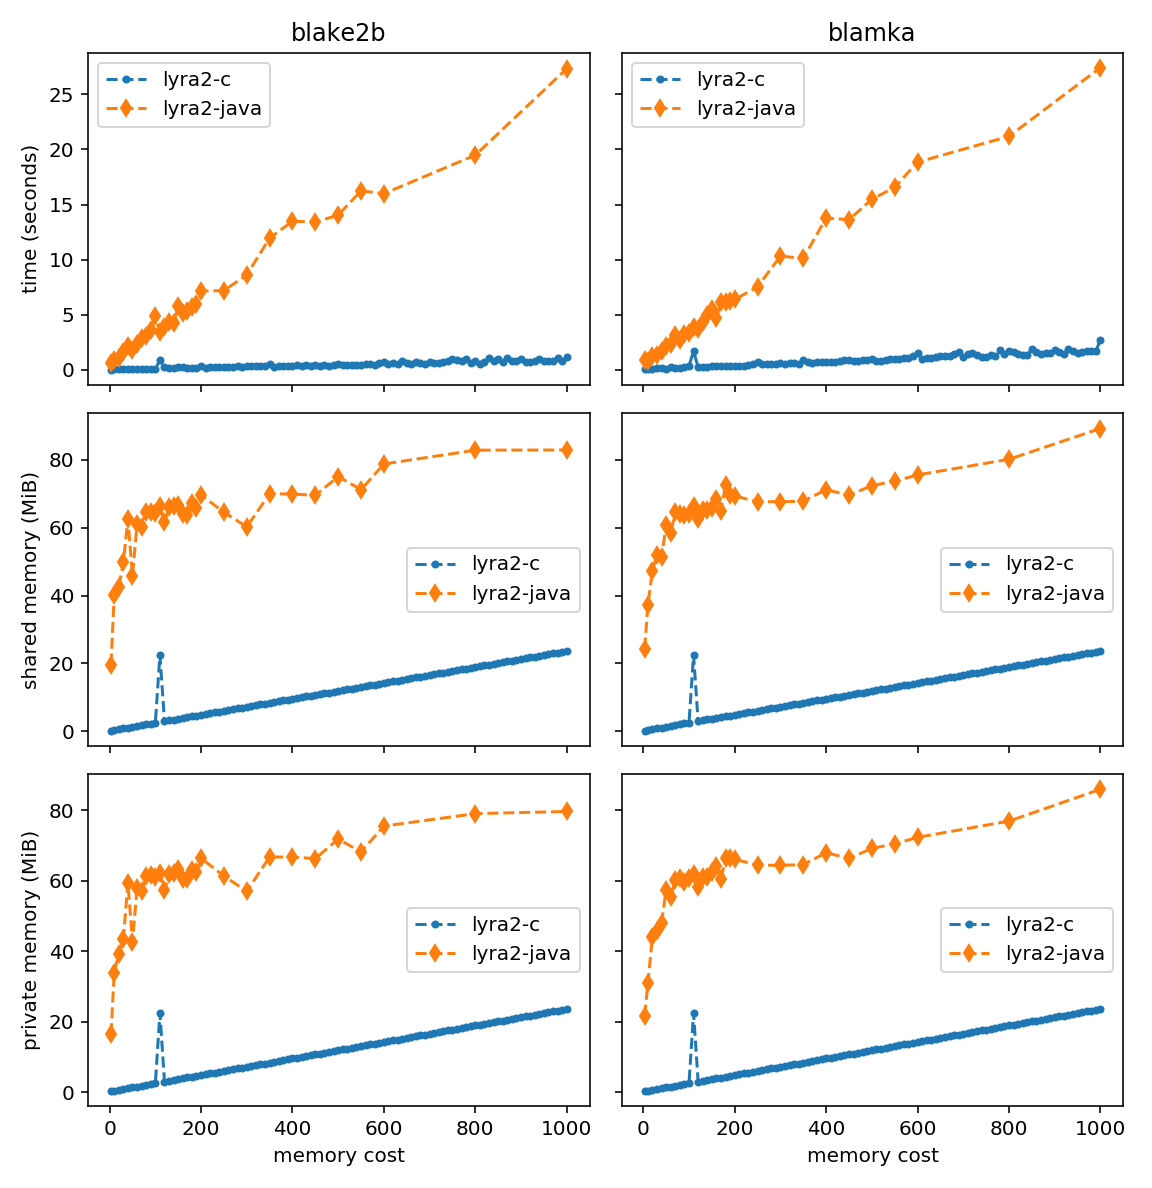
\includegraphics[width=\linewidth,keepaspectratio]{figures/mcost_256}
    \caption{\texttt{lyra2-c} compared to \texttt{lyra2-java}: 256 columns, fixed time cost of 10. Blake2b sponge on the left, BlaMka sponge on the right.}
    \label{figure:mcost_256}
\end{figure}

\begin{figure}[H]
    \centering
    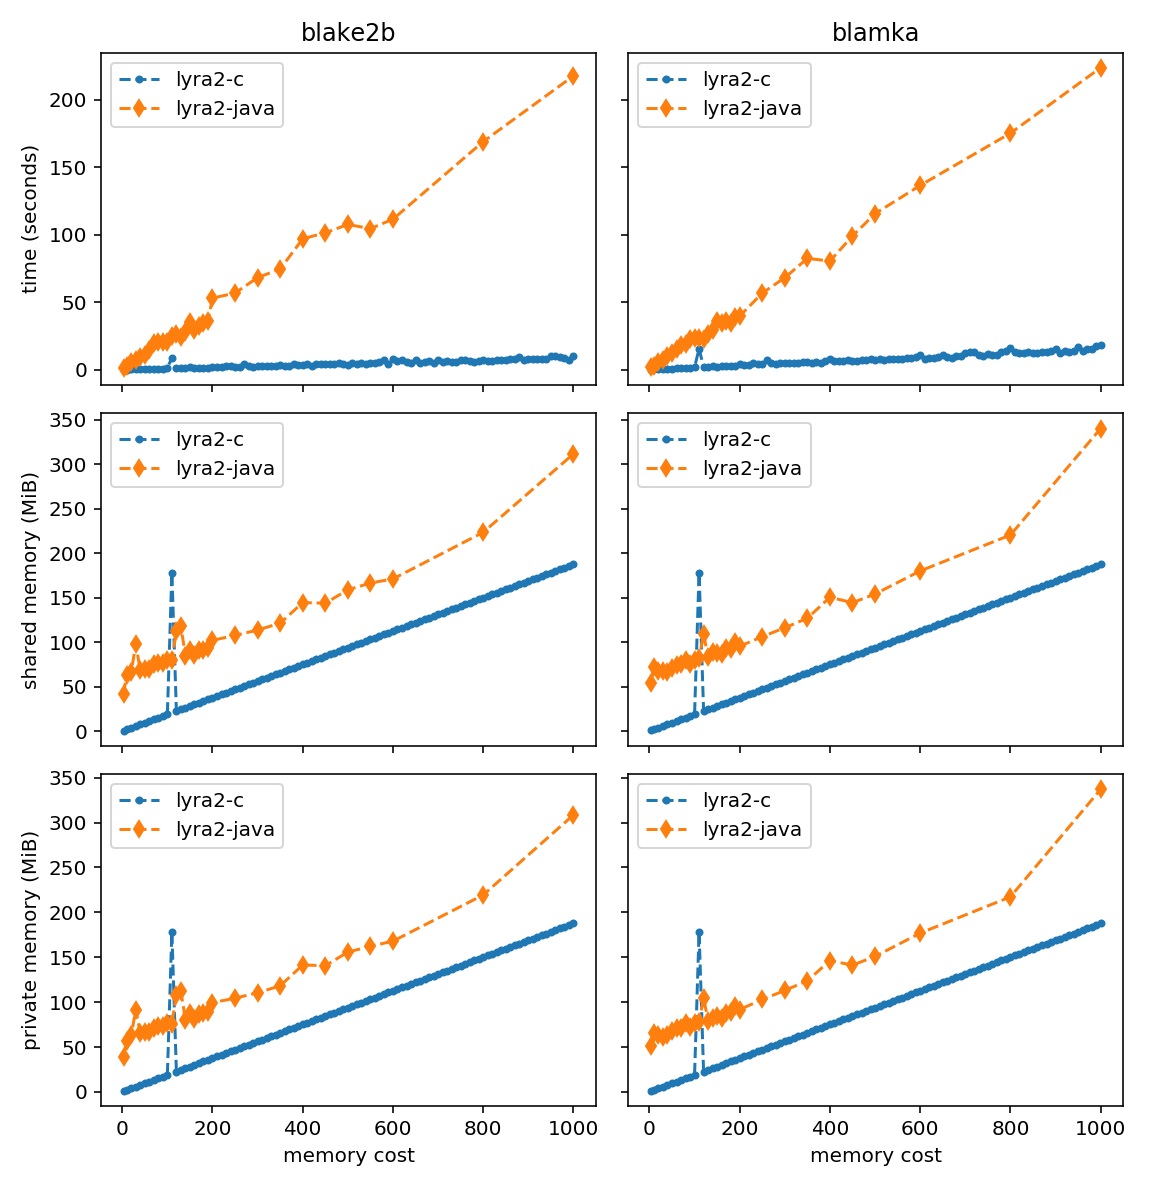
\includegraphics[width=\linewidth,keepaspectratio]{figures/mcost_2048}
    \caption{\texttt{lyra2-c} compared to \texttt{lyra2-java}: 2048 columns, fixed time cost of 10. Blake2b sponge on the left, BlaMka sponge on the right.}
    \label{figure:mcost_2048}
\end{figure}

\subsection{Fixed Memory Cost}
\label{sec:fixed-memory-cost}

There are two figures that show how running time and consumed memory depend on time cost when memory cost is fixed. Figure \ref{figure:tcost_256} shows a 256-column and figure \ref{figure:tcost_2048} shows a 2048-column configuration of Lyra2. Both these figures show that the original C implementation works faster and consumes less memory than its Java counterpart. The running time changes roughly linearly as the time cost parameter is changed which is consistent with the fact that time cost corresponds to the number of iterations done by Lyra2. Memory consumption stays roughly the same which is also consistent with the fact that the largest memory consumer is the in-memory matrix. This matrix has the same size for all of the configurations. Admittedly, there are some deviations in memory consumption of the Java implementation. The second set of figures \ref{figure:tcost_2048} even has a slight downward trend. The possible reasons for that include: the built-in garbage collector and the fact that the measurements run for several days, resulting in potentially different system loads.

\begin{figure}[H]
    \centering
    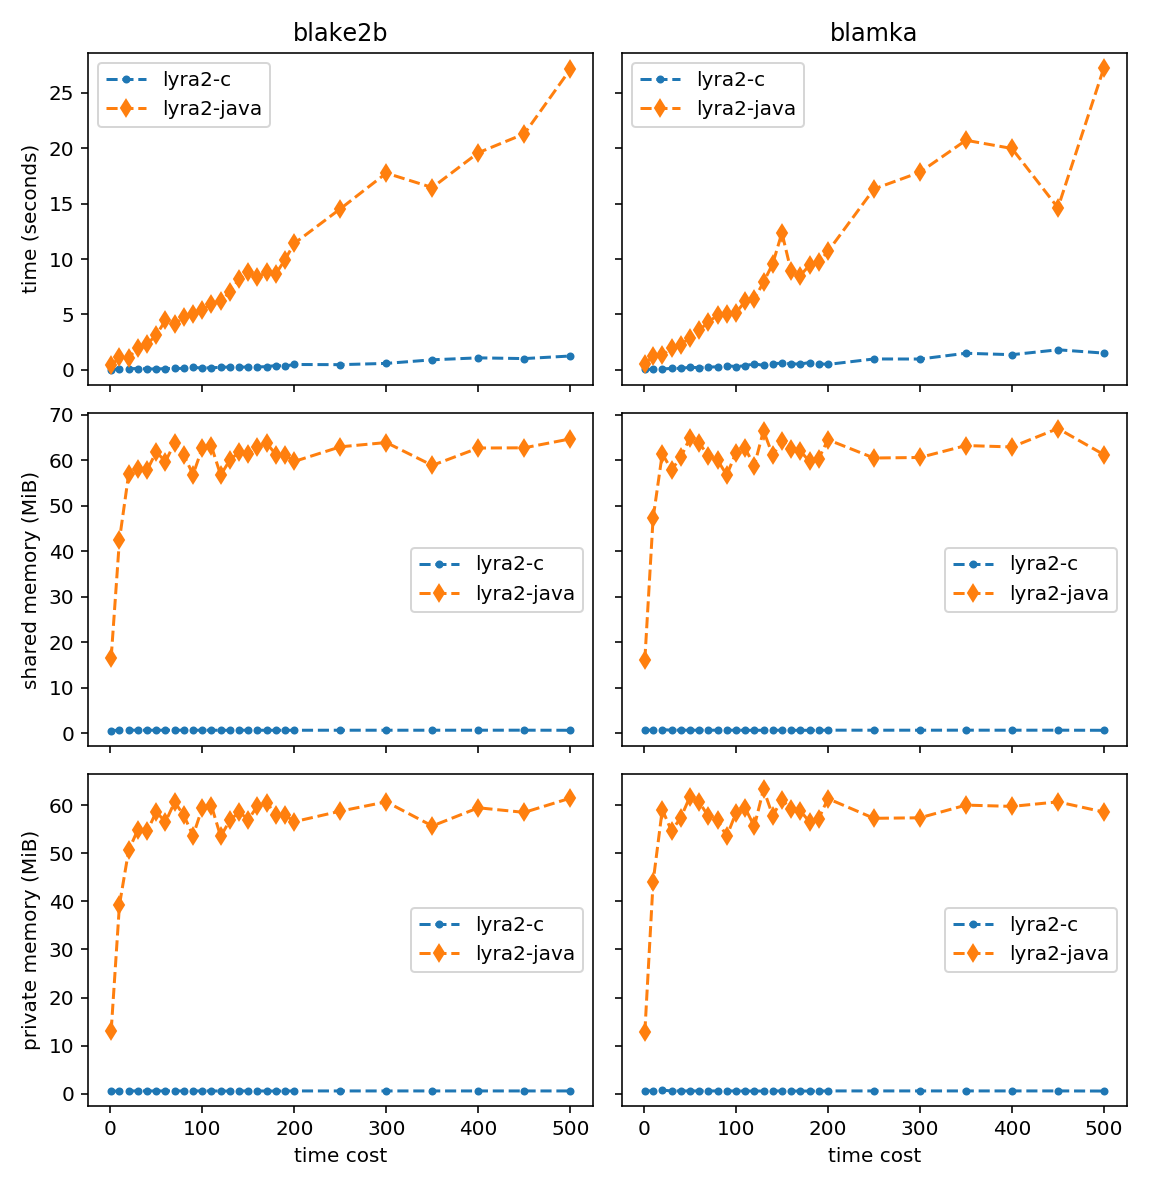
\includegraphics[width=\linewidth,keepaspectratio]{figures/tcost_256}
    \caption{\texttt{lyra2-c} compared to \texttt{lyra2-java}: 256 columns, fixed memory cost of 20. Blake2b sponge on the left, BlaMka sponge on the right.}
    \label{figure:tcost_256}
\end{figure}

\begin{figure}[H]
    \centering
    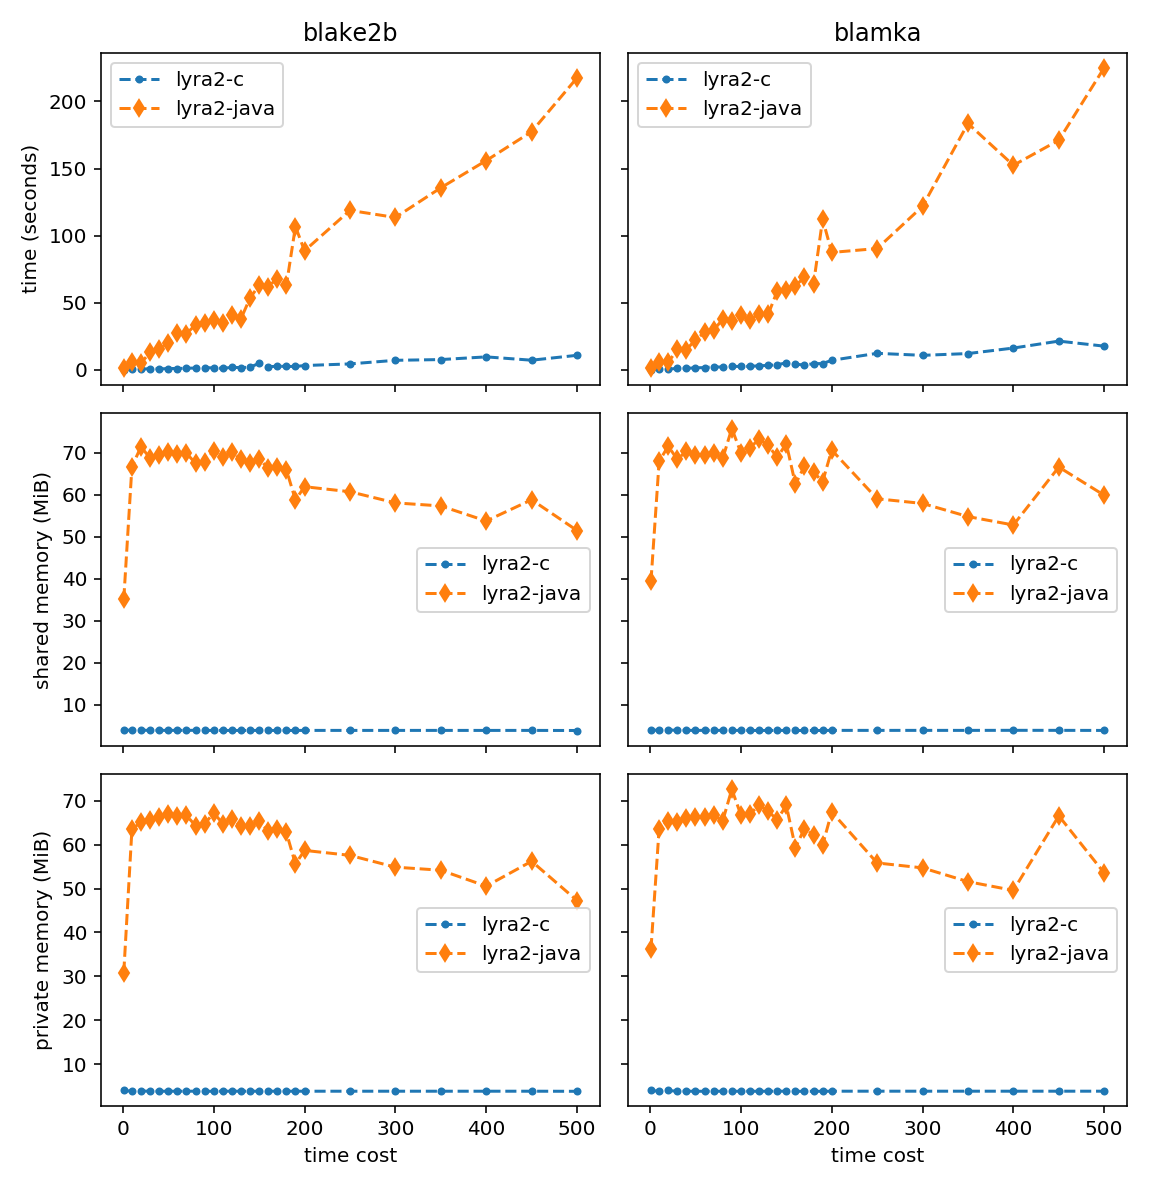
\includegraphics[width=\linewidth,keepaspectratio]{figures/tcost_2048}
    \caption{\texttt{lyra2-c} compared to \texttt{lyra2-java}: 2048 columns, fixed memory cost of 20. Blake2b sponge on the left, BlaMka sponge on the right.}
    \label{figure:tcost_2048}
\end{figure}

\subsection{Variable Time and Memory Costs}
\label{sec:no-fixed-costs}

There are four figures that show running time and memory consumption of Lyra2 when both time and memory costs change. Figures \ref{figure:tcost_mcost_blake2b_256} and \ref{figure:tcost_mcost_blake2b_2048} correspond to a 256- and 2048-column configurations of Lyra2 that both use the Blake2b sponge. Figures \ref{figure:tcost_mcost_blamka_256} and \ref{figure:tcost_mcost_blamka_2048} are the 256- and 2048-column configurations of Lyra2 with the BlaMka sponge. All of these four figures share the same properties. First of all, the reference implementation is faster and consumes less memory than its Java counterpart. Secondly, the running time as well as required space depend roughly linearly on the time and memory cost parameters. However, together they create a quadratic time growth during the \emph{Wandering phase}. This still allows for predictable and fine-tuned control of the time and memory resources required by the algorithm.

\begin{figure}[p]
    \centering
    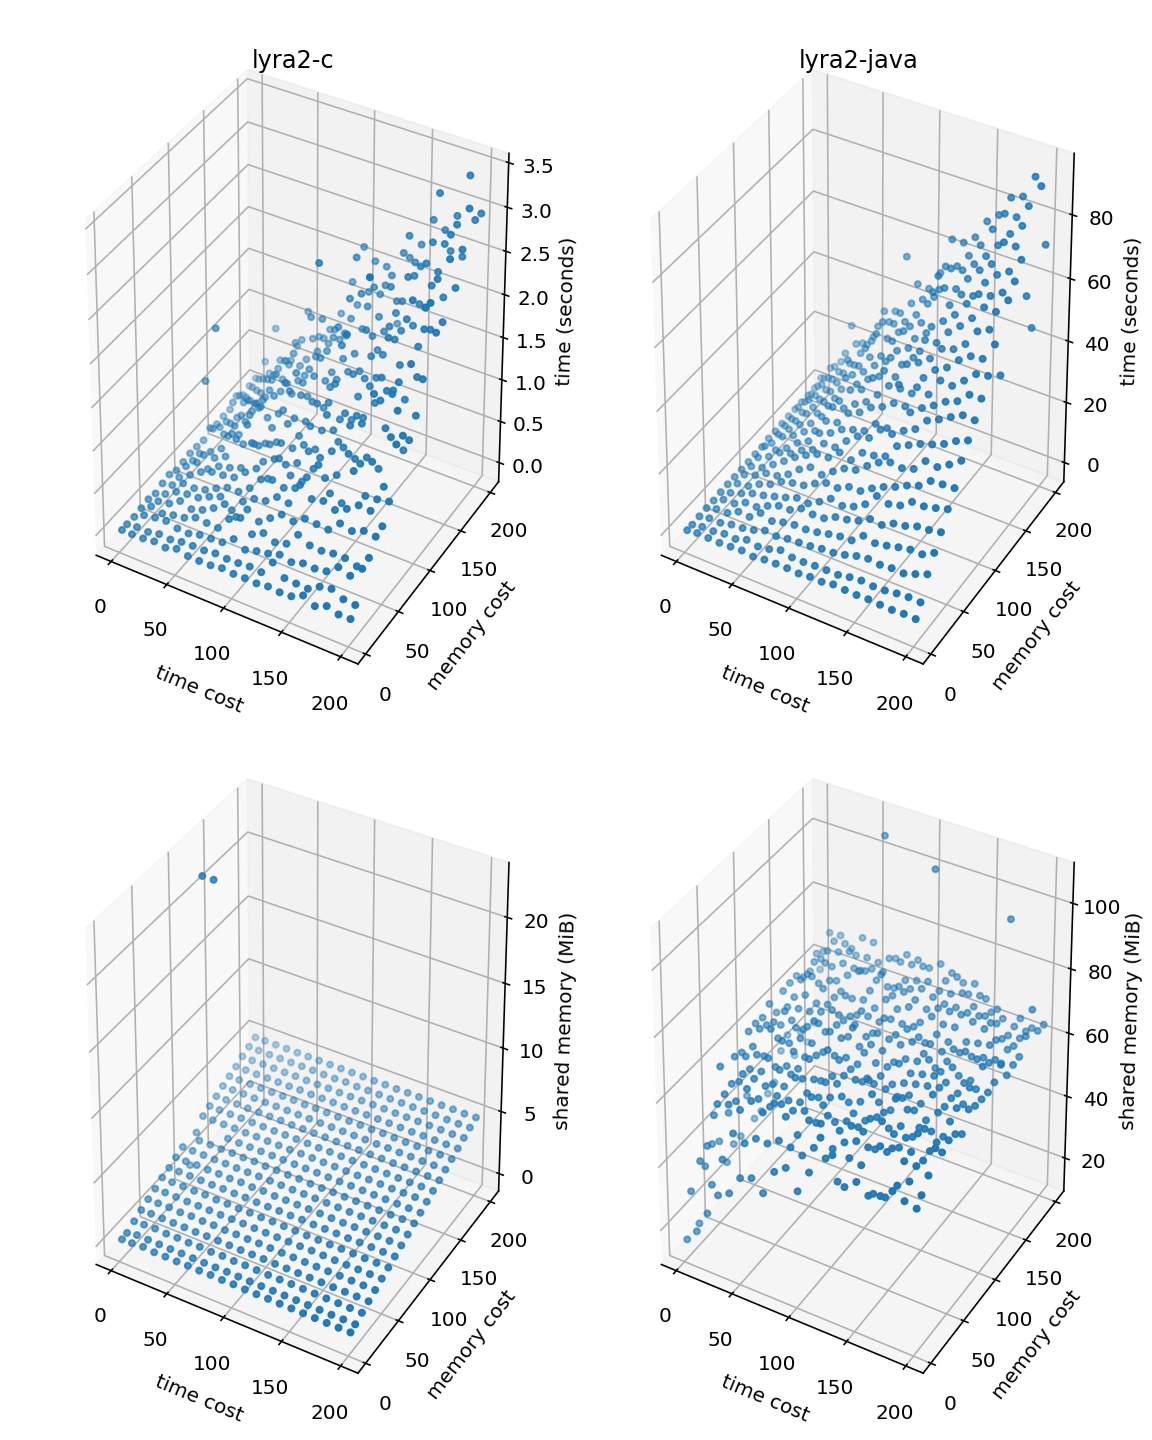
\includegraphics[width=\linewidth,keepaspectratio]{figures/tcost_mcost_blake2b_256}
    \caption{\texttt{lyra2-c} compared to \texttt{lyra2-java}: Blake2b sponge, 256 columns.}
    \label{figure:tcost_mcost_blake2b_256}
\end{figure}

\begin{figure}[p]
    \centering
    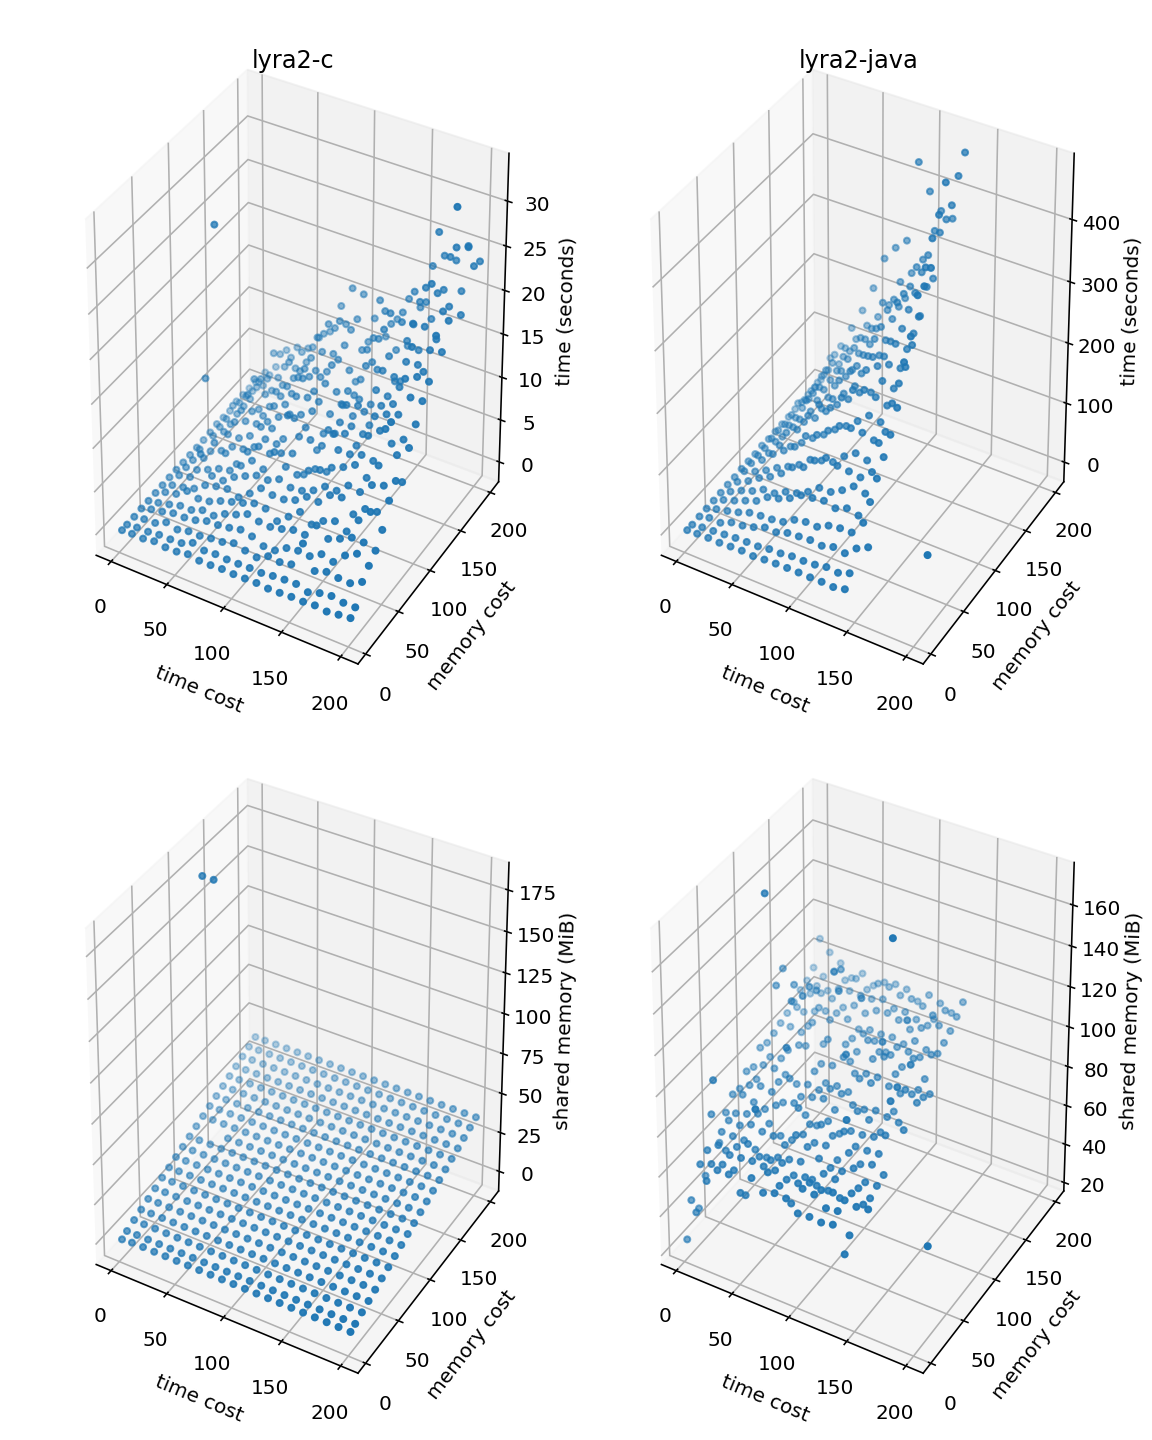
\includegraphics[width=\linewidth,keepaspectratio]{figures/tcost_mcost_blake2b_2048}
    \caption{\texttt{lyra2-c} compared to \texttt{lyra2-java}: Blake2b sponge, 2048 columns.}
    \label{figure:tcost_mcost_blake2b_2048}
\end{figure}

\begin{figure}[p]
    \centering
    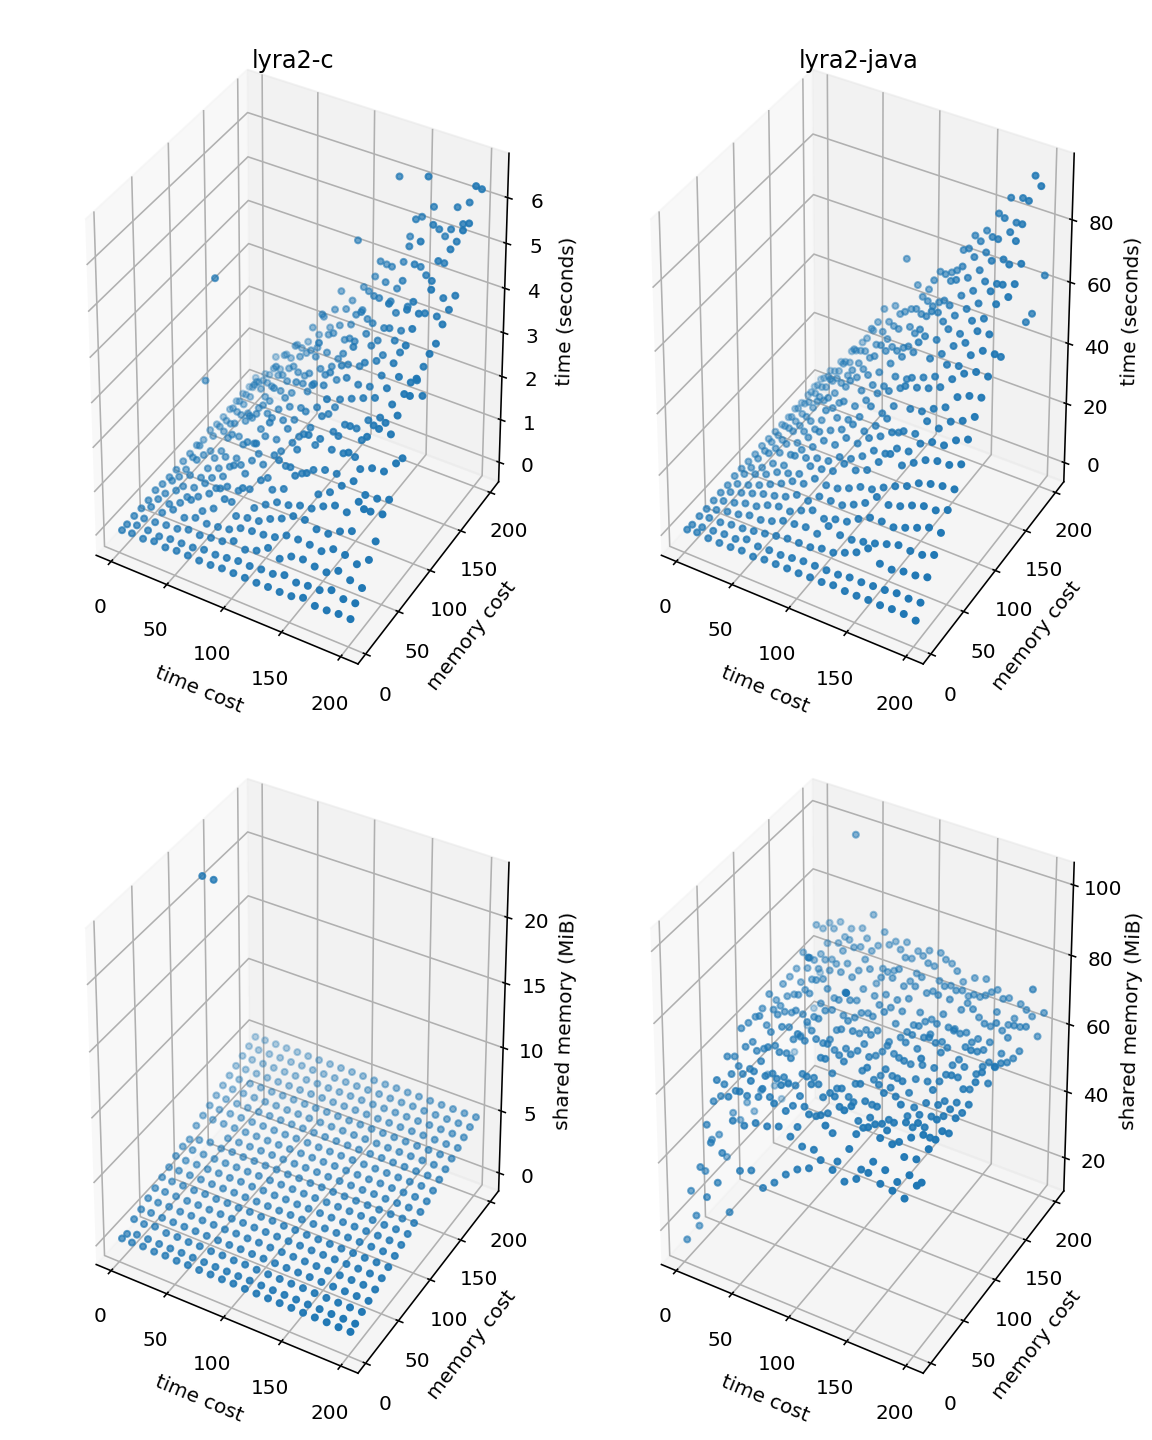
\includegraphics[width=\linewidth,keepaspectratio]{figures/tcost_mcost_blamka_256}
    \caption{\texttt{lyra2-c} compared to \texttt{lyra2-java}: BlaMka sponge, 256 columns. }
    \label{figure:tcost_mcost_blamka_256}
\end{figure}

\begin{figure}[p]
    \centering
    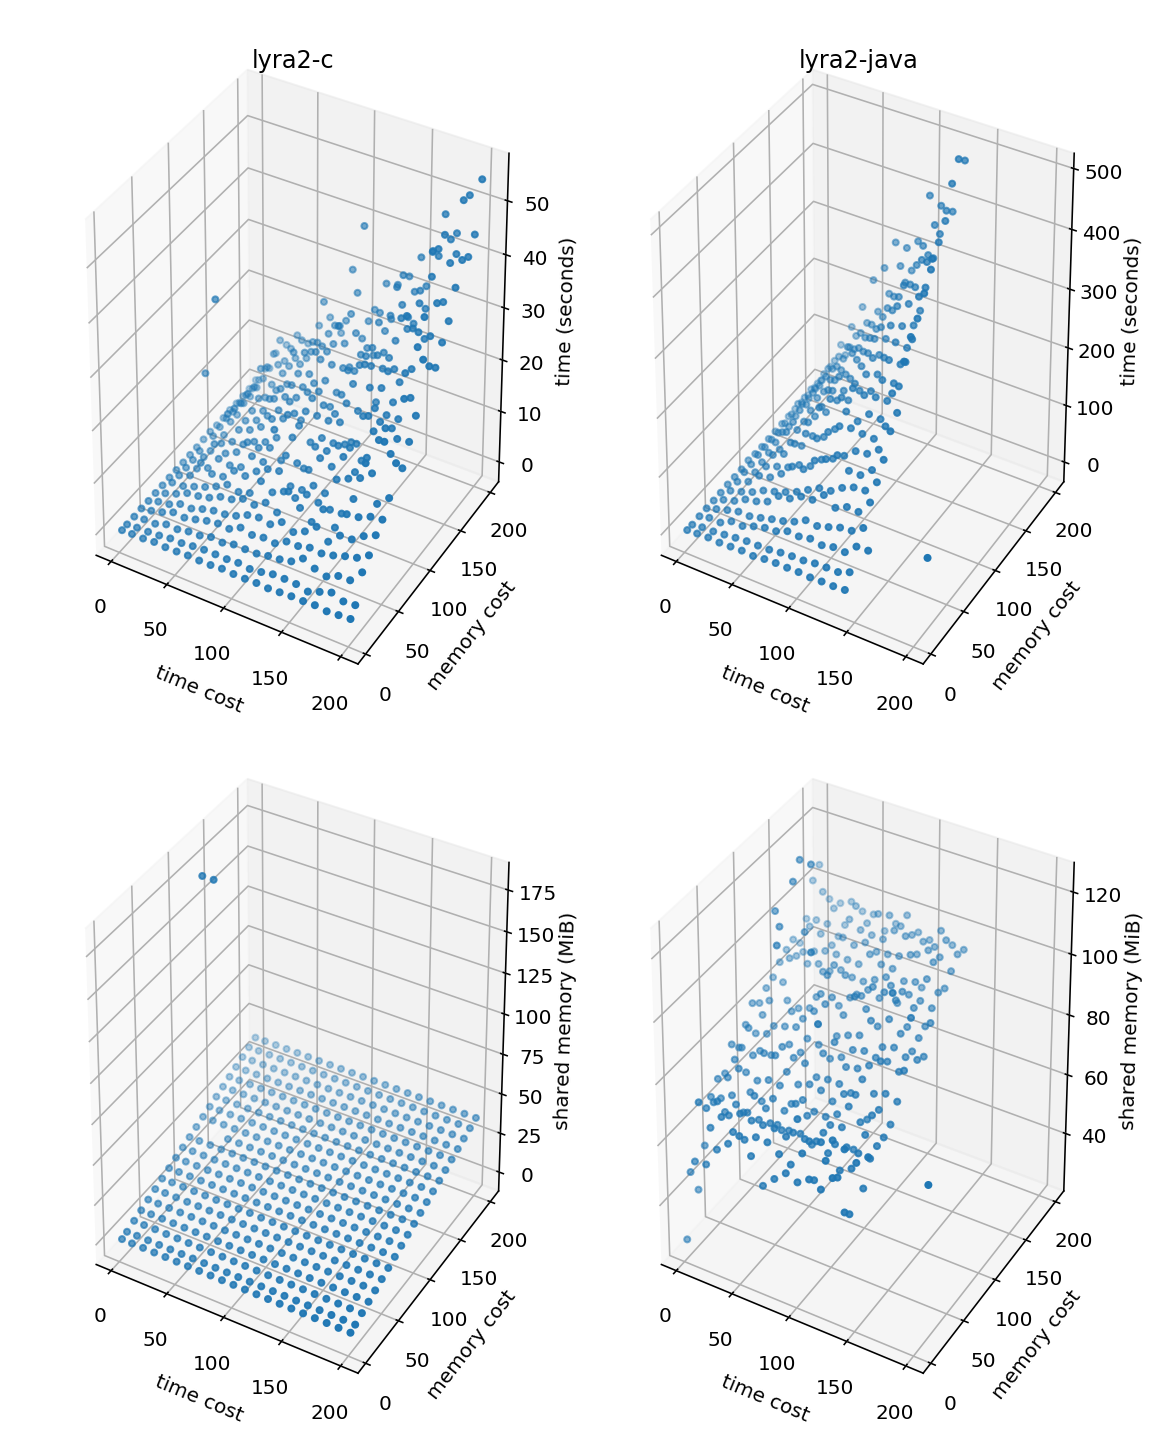
\includegraphics[width=\linewidth,keepaspectratio]{figures/tcost_mcost_blamka_2048}
    \caption{\texttt{lyra2-c} compared to \texttt{lyra2-java}: BlaMka sponge, 2048 columns.}
    \label{figure:tcost_mcost_blamka_2048}
\end{figure}

\clearpage
\subsection{Comparison Conclusion}
\label{sec:comparison-conclusion}

The Java implementation was outperformed by the reference C implementation. This could in part be attributed to language ecosystems or programming skills but it also cannot be denied that the ported version takes a lot of extra steps in order to ensure algorithm-level compatibility. These include the extra rotations required to simulate little-endian behavior, as well as simulating pointer arithmetic and unsigned arithmetic for large 64-bit integers.

\section{Android Application}
\label{sec:mobile-application}

Part of the porting effort is a small proof of concept mobile application. This application demonstrates that using a native Java library in an Android project is convenient.

One of the first steps is to determine the minimum versions of Android devices and API levels necessary. Since lyra2-java makes use of unsigned 64-bit number arithmetic, Java 1.8 support is required. This translates into the minimum Android version of 7.0 and the API level of 24 \cite{android:2017:java-support}.

One of the most common development environments for Android applications is the Android Studio. Support for Java 1.8 features has not yet landed into the release version of this IDE. So, in order to be able to develop a mobile application with Lyra2, a development version \texttt{3.0} needs to be installed. If you encounter a (similar) traceback as shown in \autoref{fig:traceback}, one possible workaround is to instruct Android Studio to use system libraries:

\begin{minted}{shell}
ANDROID_EMULATOR_USE_SYSTEM_LIBS=1 ./studio.sh
  \end{minted}

\begin{code}
\begin{minted}{shell}
    Emulator: libGL error: unable to load driver: i965_dri.so
    Emulator: libGL error: driver pointer missing
    Emulator: libGL error: failed to load driver: i965
    Emulator: libGL error: unable to load driver: i965_dri.so
    Emulator: libGL error: driver pointer missing
    Emulator: libGL error: failed to load driver: i965
    Emulator: libGL error: unable to load driver: swrast_dri.so
    Emulator: libGL error: failed to load driver: swrast
    Emulator: X Error of failed request:  BadValue (integer parameter out of range for operation)
    Emulator: Major opcode of failed request:  155 (GLX)
    Emulator: Minor opcode of failed request:  24 (X_GLXCreateNewContext)
    Emulator: Value in failed request:  0x0
    Emulator: Serial number of failed request:  42
    Emulator: Current serial number in output stream:  43
    Emulator: Process finished with exit code 1
\end{minted}
\caption{Android Studio emulator: an obscure error traceback connected to \texttt{libGL}.}
\label{fig:traceback}
\end{code}

Once these preliminary steps are performed, the development of the application becomes straightforward. Android Studio is based on IntelliJ Studio and therefore picks up lyra2-java from the Maven Central repository in a matter of a couple clicks.

As a result, a simple Android application was developed and is available on GitHub \cite{github:2017:lyra2-mobile}. It consists of a main screen and a results screen. The main screen allows the user to choose some particular configuration of Lyra2. By default, the Blake2b sponge with the time and memory cost of 100 will be used. The password and salt fields are set to the default values of "password" and "salt" respectively, the number of columns is 256 with each column being 12 blocks wide. The permutation inside the sponge makes a total 12 rounds of computations. All of the parameters above can be adjusted.

\autoref{fig:lyra2-mobile-demo} summarizes the result. In particular, \autoref{fig:lyra2-mobile-main-blake2b} and \autoref{fig:lyra2-mobile-result-blake2b} show the main screen and the results screen when running Lyra2 in the mobile emulator with the default parameters. At the same time \autoref{fig:lyra2-mobile-main-blamka} and \autoref{fig:lyra2-mobile-result-blamka} show the settings and the result for the BlaMka sponge. In both cases the hash values match those from the manual testing Section \ref{sec:manual-testing}. In each case the computation lasted for approximately 60 seconds which is consistent with the desktop version times. However, it should once again be noted that the application was run in an emulator and not on an actual mobile device.

\begin{figure}[H]
\centering
\begin{subfigure}{.5\textwidth}
  \centering
  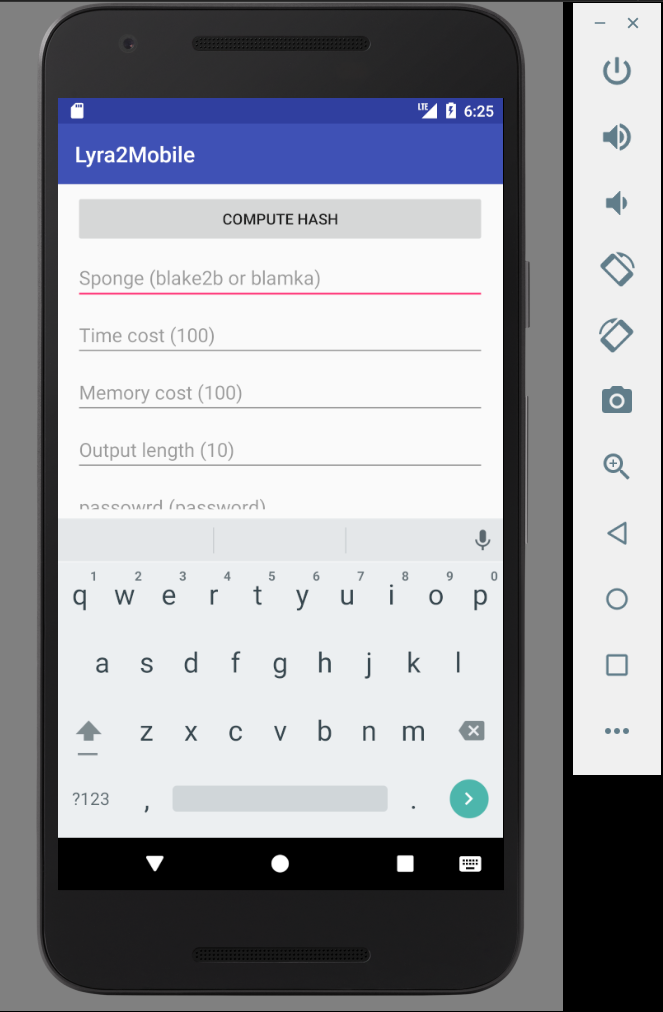
\includegraphics[width=.8\linewidth]{figures/lyra2-mobile-main-clean}
  \caption{Main screen (Blake2b sponge, default)}
  \label{fig:lyra2-mobile-main-blake2b}
\end{subfigure}%
\begin{subfigure}{.5\textwidth}
  \centering
  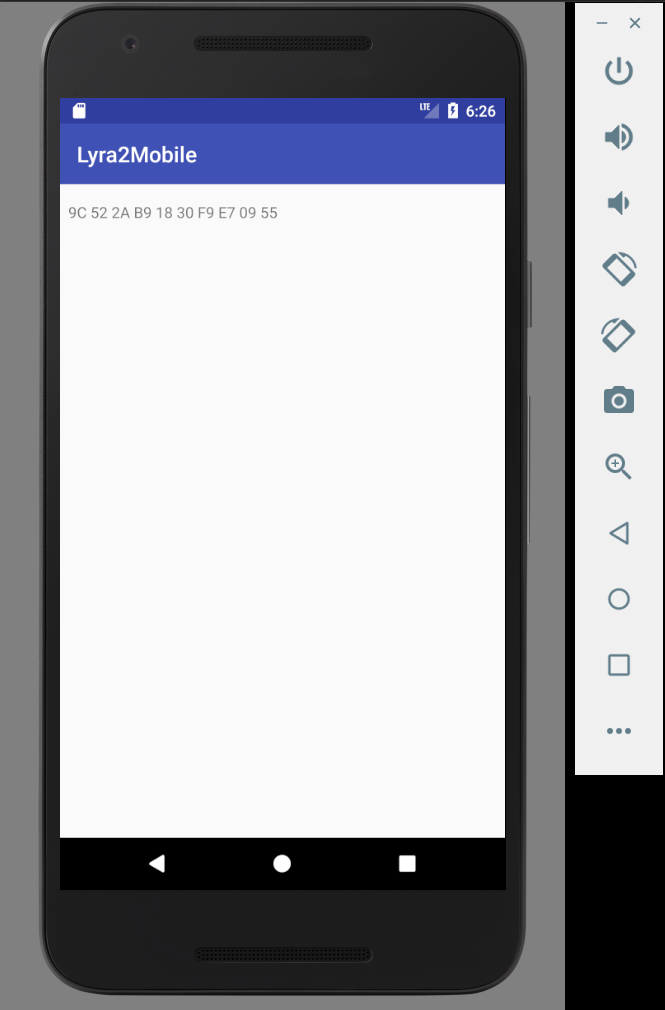
\includegraphics[width=.8\linewidth]{figures/lyra2-mobile-result-clean}
  \caption{Resulting hash (Blake2b sponge, default)}
  \label{fig:lyra2-mobile-result-blake2b}
\end{subfigure}
\begin{subfigure}{.5\textwidth}
  \centering
  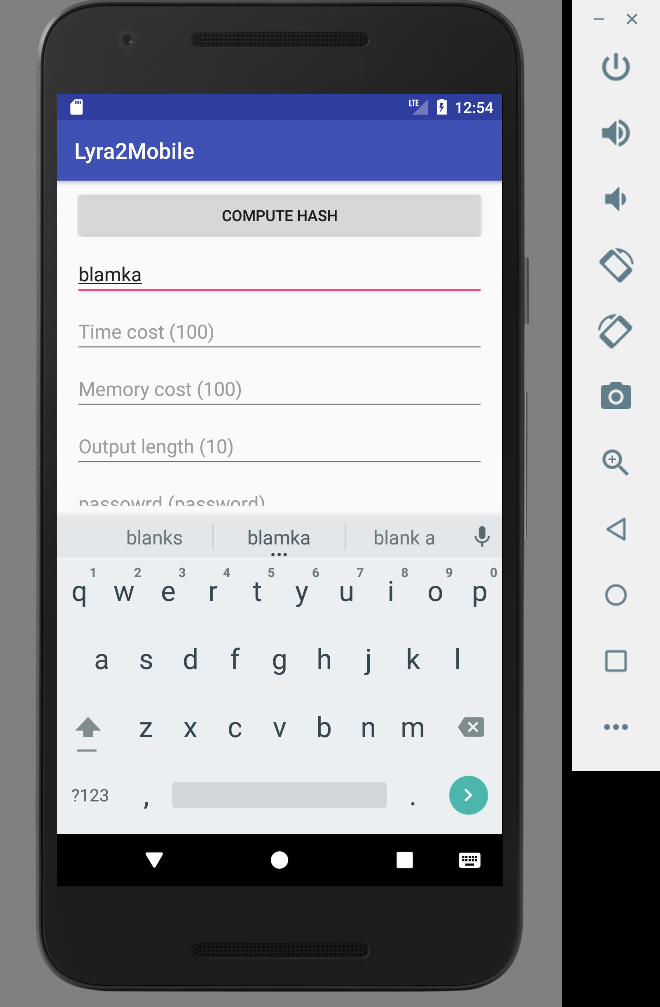
\includegraphics[width=.8\linewidth]{figures/lyra2-mobile-main-blamka-clean}
  \caption{Main screen (BlaMka sponge)}
  \label{fig:lyra2-mobile-main-blamka}
\end{subfigure}%
\begin{subfigure}{.5\textwidth}
  \centering
  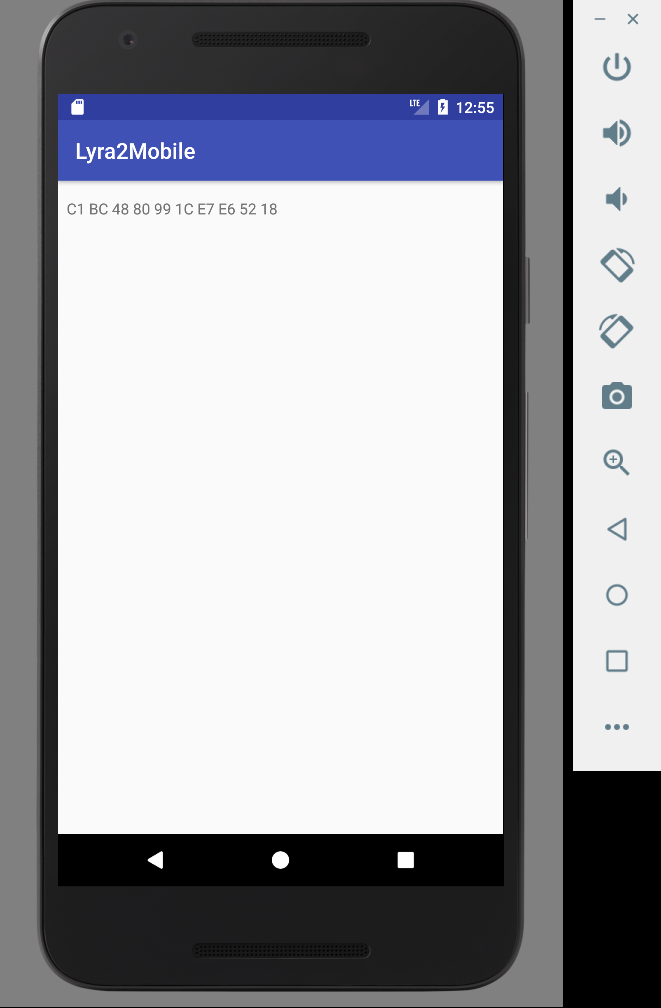
\includegraphics[width=.8\linewidth]{figures/lyra2-mobile-result-blamka-clean}
  \caption{Resulting hash (BlaMka sponge)}
  \label{fig:lyra2-mobile-result-blamka}
\end{subfigure}
\caption{Android application running Lyra2. Each of the two configurations runs for \(\approx 60\) seconds. Parameter values on the left, resulting hash in hexadecimal on the right.}
\label{fig:lyra2-mobile-demo}
\end{figure}
